\chapter[Task 16]{\#16: Traffic Congestion}

\resp{David Weingut}

\section{Overview}
This project is concerned with a simplified model of traffic on top of a network.
The simulated dynamics will follow the behaviour outlined in the research papers\cite{Echenique2004}\cite{Echenique2005}.
The system consists of a network and packets moving in this network.
The packets are simple entities, they just contain their own destination as data.
Each node of the network can hold a potentially infinite number of packets.
A packet gets effectively destroyed upon arrival at its destination.
Each time step a single packet is sent from each node that has a packet to send to one of its neighbours.
The neighbour is for a deterministic approach chosen according to equation \ref{eq:neighbour-sel-16}, where $b$ is the best next node for the packet, chosen by being the neighbour of current vertex $l$ minimizing the effective distance function $d_\mathrm{eff}$.
\begin{equation}
	b = \argmin_{i \in \{1, ..., k_l\}} d_\mathrm{eff}\left(i, \mathrm{destination}\right) \label{eq:neighbour-sel-16}
\end{equation}
The dependence of the behaviour of the system on the choice of distance function is the main interest in this project.
A naive approach would be to just follow the shortest path to the destination, so $d_\mathrm{eff}(i, j) = hd(i, j)$, with $d$ being the geodesic distance.
A possible improvement suggested in the aforementioned papers is to ``incorporate local traffic information''\cite[Abstract]{Echenique2005}.
This happens via an configurable interpolation of shortest path information and queue length for the candidate, the distance function takes the form $d_\mathrm{eff}(i, j) = hd(i, j) + (1-h) n_i$ where $n_i$ is the number of packets currently at node $i$.

The papers differ in the approach they take to the temporal distribution of the addition of packets.
I am using the approach of \cite{Echenique2005}, that a continuous influx of $p$ packets per time step (\si{\pps}) is realized and the amount of packets currently in the system is observed.
They introduce an order parameter $\rho$ describing the relative change of active packets.
\begin{equation}
	\rho = \lim_{t\rightarrow\infty} \frac{A(t+\tau) - A(t)}{\tau p}
\end{equation}
It takes values in the range 0, a stationary state meaning free flow, and 1, no packages reach their destination, total congestion.

In the following I will investigate the behaviour of the dynamics for different network topologies.

\section{Random Graphs}
A first idea was to test different routing strategies on different types of random graphs like Erdös-Renyi or Watts-Strogatz based ones.
This idea was then discarded again when I read that the behaviour was strongly dependent on the exact clustering of the graph\cite[p.~2]{Echenique2005} and after I discovered in some preliminary simulations that the spread of the active packets is quite large even for the same exact network.
In connection with wanting to fairly represent the ensemble I thought it too computationally complex to get a faithful estimate of the performance across both graphs in an ensemble and different simulation runs for one topology.

\section{Autonomous System Maps}\label{sec:ASmaps-16}
For this reason I decided that I would take a real network, inspired by the original papers and motivations for the algorithm chosen to be an autonomous system map.
The one I chose is from 29 December 1998, collected for \cite{OregonAS} and downloaded from \cite{snapnets}.
It has \num{493} nodes and \num{1234} edges with an average clustering coefficient of \num{0.1756} and a diameter of \num{8} hops.

\begin{figure}[h]
	\centering
	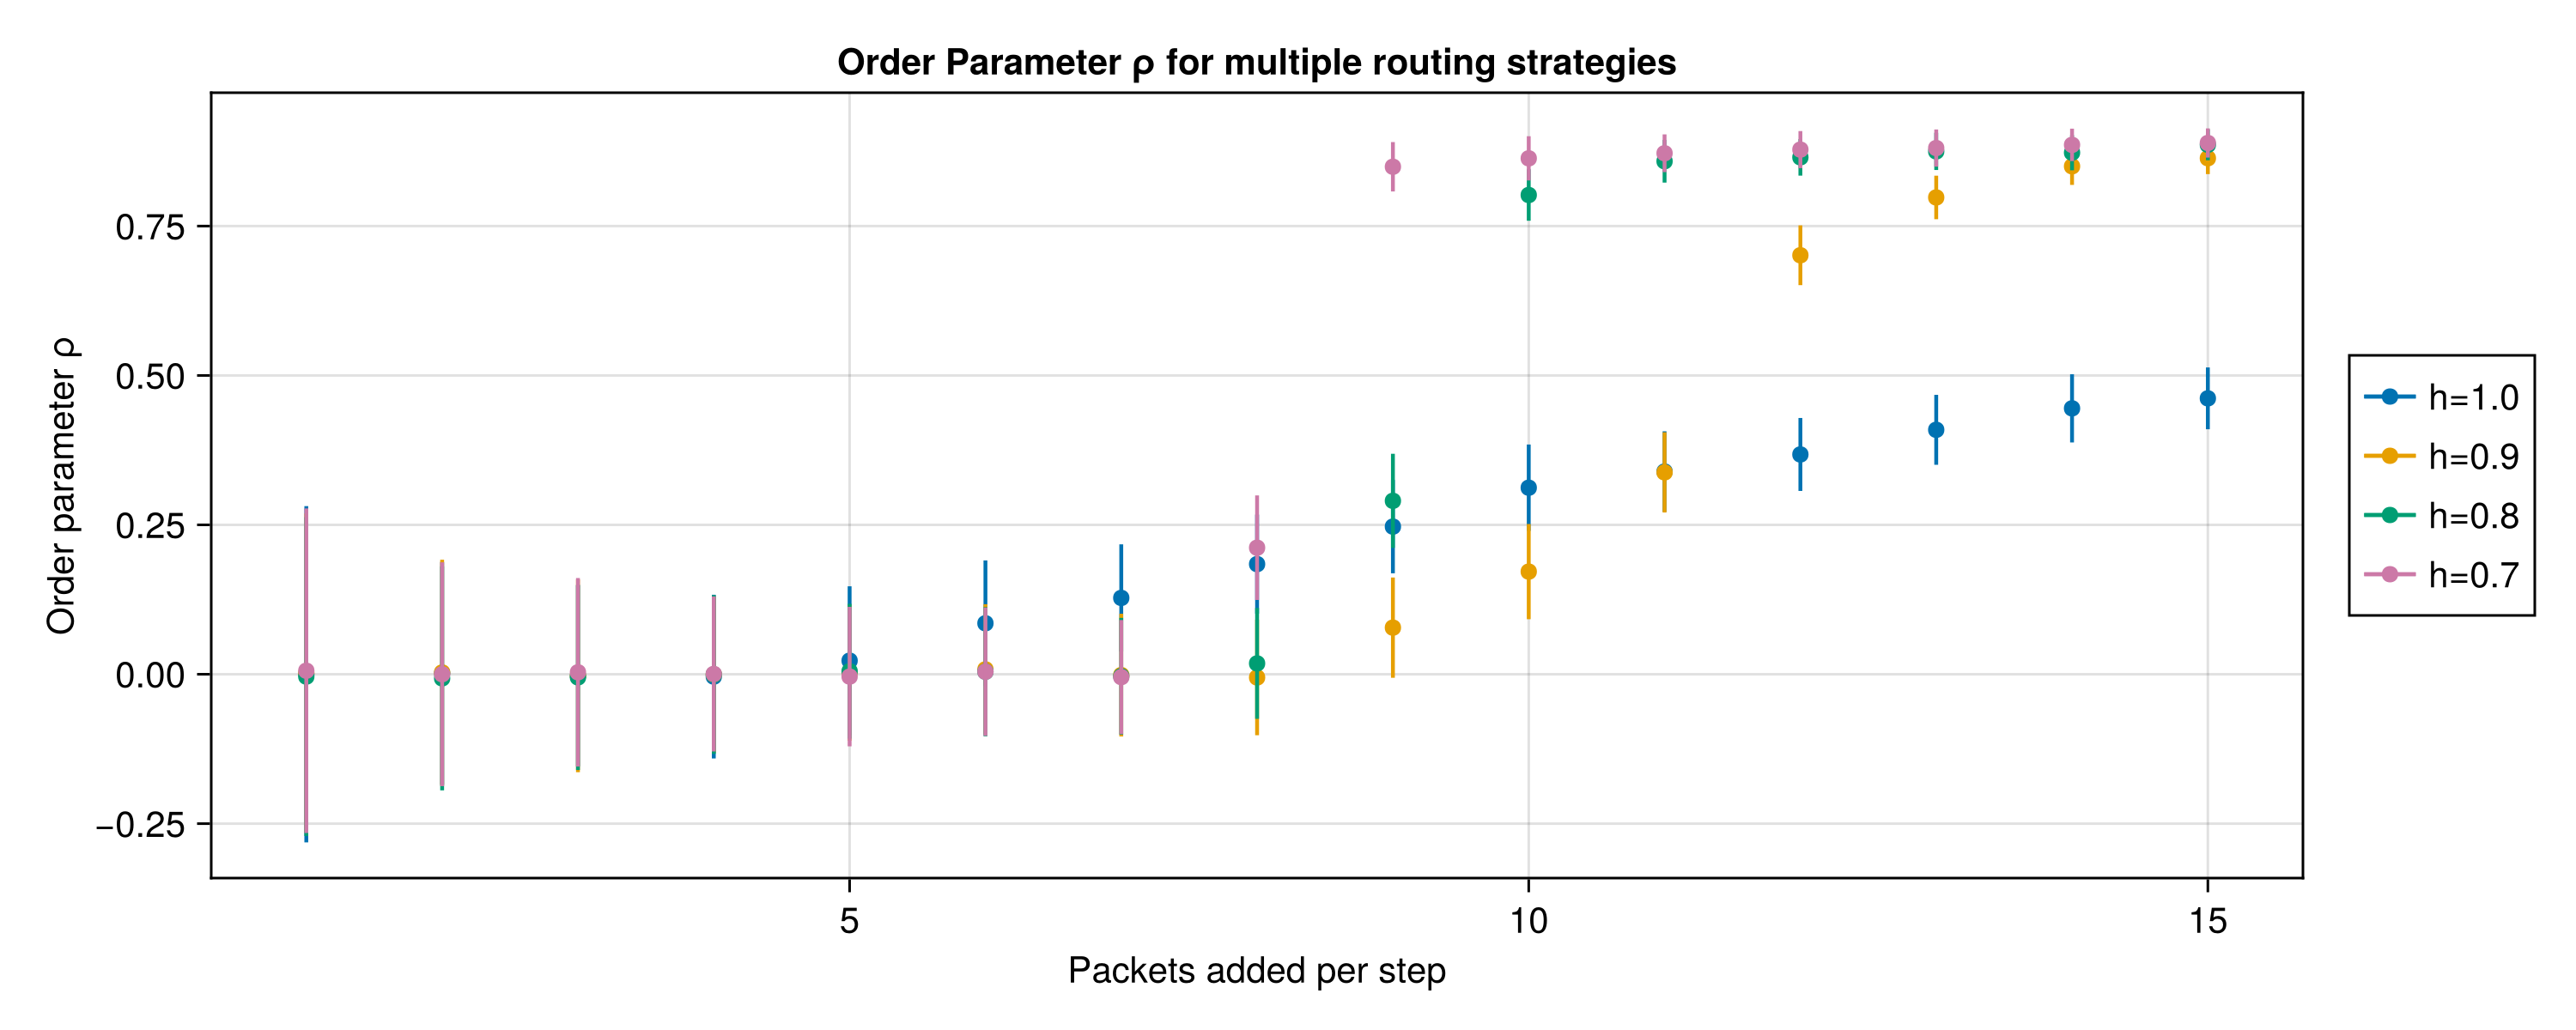
\includegraphics[width=\textwidth]{reduced_plot_h_pps}
	\caption{Comparison of neighbour choice algorithms. More details in the text.}
	\label{fig:neighbour-16}
\end{figure}

The behaviour depending on the weight of the path length vs the queue length can be seen in figure \ref{fig:neighbour-16}.
It can be clearly seen that for high package creation rates the choice based only on the shortest path is the one which handles it most effectively, even though there still is a growth of the active packet count by almost half the input rate, the network seems to be over-saturated.
For the queue length aware algorithms there is an area between \SI{5}{\pps} and \SIrange{8}{10}{\pps}, depending on the exact value of $h$, where they reign superior.
This increased performance however rapidly increases if a certain threshold is crossed.
While $h=1$ needs \num{4} more packets to reach $\rho=\num{0.25}$ after initially departing from \num{0} while for $h=0.7$ it only takes \num{2} packets to go from $\rho\approx\num{0}$ at \SI{7}{\pps} to reach $\rho>\num{0.75}$ for \SI{9}{\pps}. For higher values of $h$ the transition is more gradual and comes later.
The nature of the phase transition agrees with \cite{Echenique2005} while they didn't find a correlation of $h$ with the onset of it.

\section{Elementwise Application}
As an additional idea I wanted to test if there was any difference in behaviour if the effective distance according to equation \ref{eq:neighbour-sel-16} would not be applied during the final step but during the search for the shortest path. For this I applied the respective distance function to each element of the weight matrix. This made the graph into a weighted graphs where the edge weights are constantly changing according to the number of packets residing in the target node of the edge. This will be called the element wise approach in the following.
For computational reasons I used the smallest network in the dataset I used in section \ref{sec:ASmaps-16}. This network is from 29 August 1999 has \num{103} nodes and \num{248} edges with an average clustering coefficient of \num{0.2703} and a diameter of \num{6} hops.

\begin{figure}[h]
	\centering
	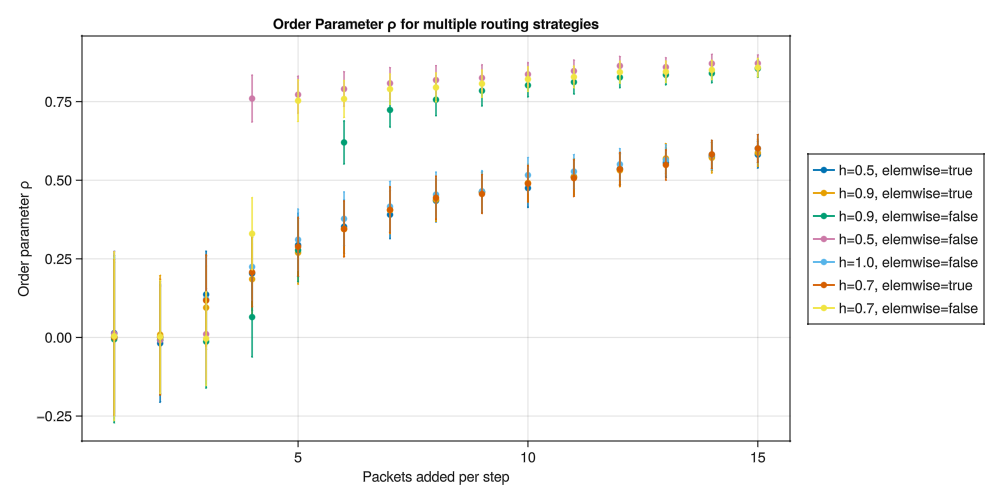
\includegraphics{reduced_plot_h_elemwise_pps_notfirst}
	\caption{Comparison of different path length modifiers and neighbour choice algorithms. More details in the text.}
	\label{fig:elemwise-16}
\end{figure}

The results can be seen in figure \ref{fig:elemwise-16}.
For this simulation run I chose to use the aforementioned adjusting of the weights wherever the label in the legend says \texttt{elemwise=true}.
Here the change of single weights in turn used just the length of the shortest path found by the weighted search algorithm, the neighbour selection was greedy and not taking into account the traffic information at the next node, only on its further path.
The performance of these modified protocols were within the margin of error identical to the protocol that completely disregards traffic information.
In figure \ref{fig:elemwise-allscaled-16}, shown in the appendix, the original behaviour as described in equation \ref{eq:neighbour-sel-16} was kept additionally to adding traffic information along the path.
Here the element wise approach's performance was pretty much indiscernible from the one without my addition.
In conjunction these figures seem to imply that the choice of the next node to travel to is the most important one while the traffic information later in the path has a negligible impact.
This may be connected to the unpredictable nature of the traffic in this scenario as while you look at the second next node, there could be up to $k-1$ more packets waiting for delivery.
I did not look at the detailed behaviour of the model for this algorithm, the crowding behaviour in connection to the betweenness centrality as done in \cite{Echenique2005} may be an interesting avenue for further research.
In total I would say the additional computational complexity of the approach described in this section is not worth it for unclear gains.

\newpage